\chapter{Work Completed}\label{C:work}

Concrete work done is as follows\dots

Overview of design and approach and any initial starting design decisions. 

\section{Substrate Mounting}
The proposal initially outlined the design mount/fastener for the substrate stack, to intergrade a heat spreader, better ensure cantering and thermocouple placement. Initial meetings (with workshop) and design started early with rough sketch designs and discussions on material and manufacture. However, it was quickly decided that focus should be shifted elsewhere in the project and this be returned to at a later date if needed, as the substrate is a shared component of the 2 projects centred around this experimental setup and the development new droplet dispensing was the true focus of this project.

\section{Pipette and Mechanical Mounting}
Given the decision for the new rig to be centred around an electronic (as apposed to the manual syringe) a new mounting assembly was needed to secure the pipette to the XYZ stage, ensure there is minimal play/backlash and position its tip above the substrate for droplet dispensing.

\begin{figure}
    \centering
    \begin{subfigure}{.3\textwidth}
      \centering
      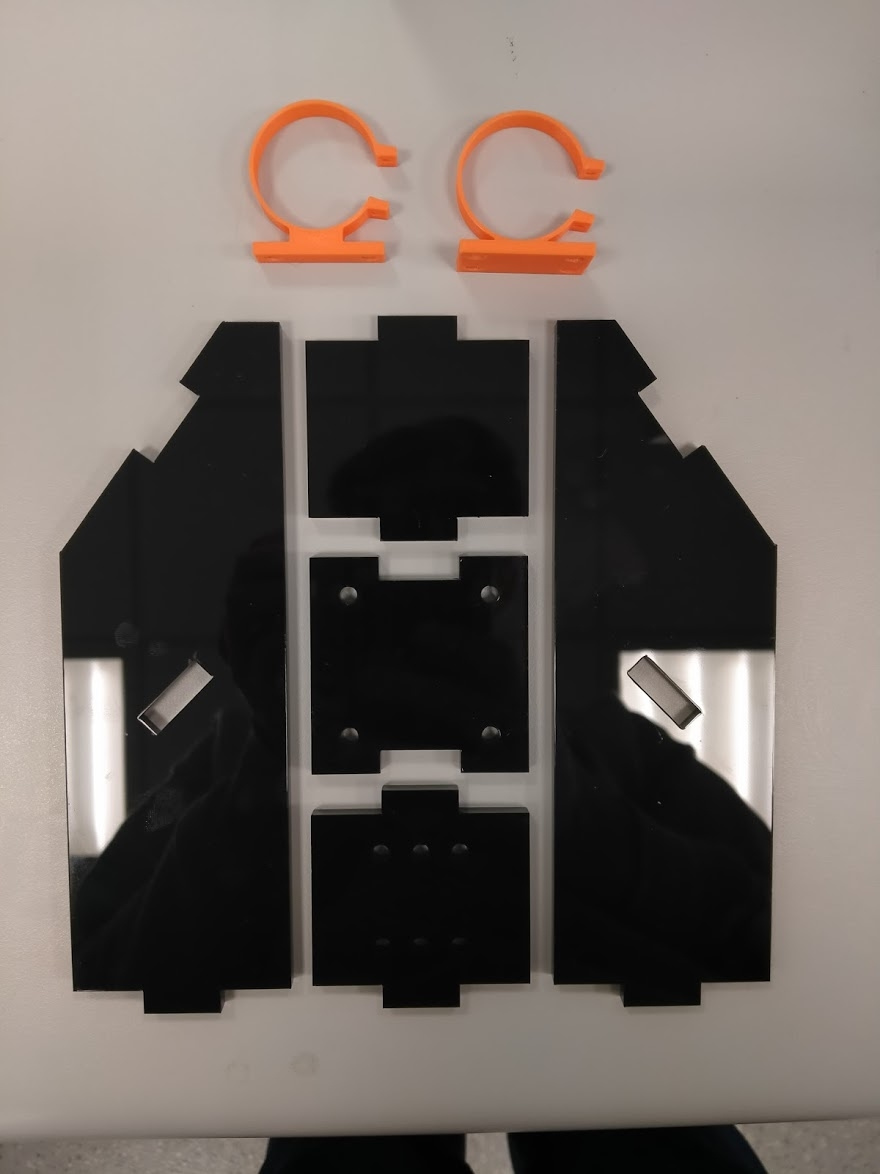
\includegraphics[height=\linewidth]{img/Tower_pcs.jpg}
      \caption{Unassembled Tower}
    \end{subfigure}%
    \begin{subfigure}{.3\textwidth}
      \centering
      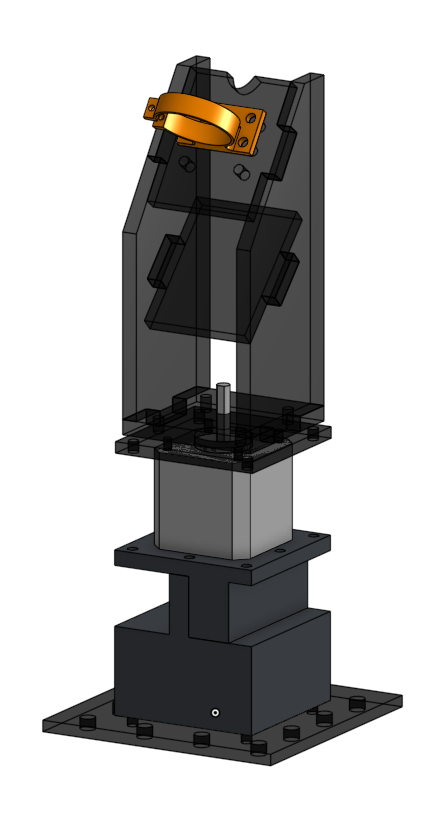
\includegraphics[height=\linewidth]{img/motor_cad_mouting.png}
      \caption{CAD Design}
    \end{subfigure}
    \begin{subfigure}{.3\textwidth}
        \centering
        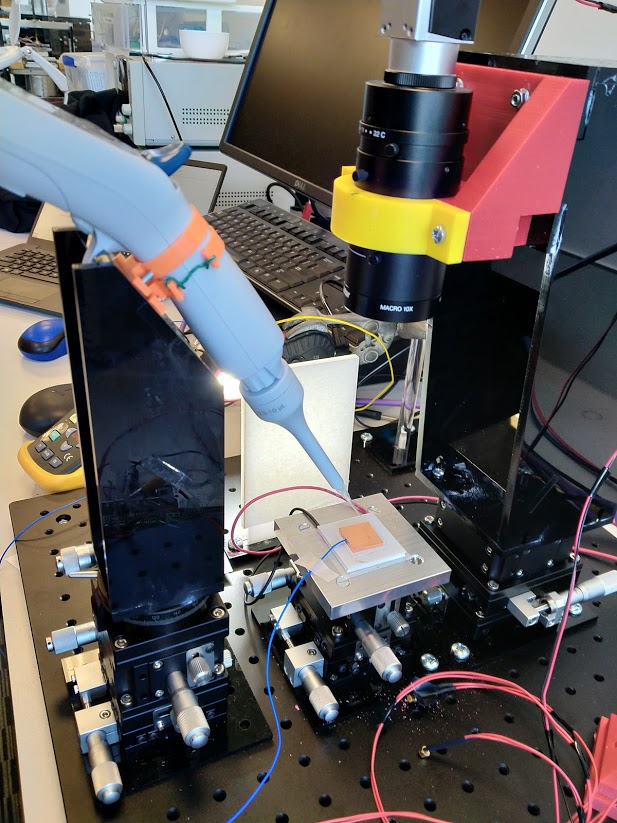
\includegraphics[height=\linewidth]{img/Tower_ass.jpg}
        \caption{Tower Assembled}
      \end{subfigure}
    \caption{Pipette Tower}
    \label{fig:tower}
  \end{figure}

\textbf{Requirements:} The pipette had to be held at 150mm from the top of the optical stage, at 36 degrees. Finer adjustments to be made with the XYZ micrometre controls. 

A tower [\ref{fig:tower}] was designed as the mounting solution. It was constructed from laser cut 6mm acrylic as it had been successfully used in other parts of the existing rig, could be very quickly manufactured to allow rapid prototyping and producing a variety of mounting points and different plates. Assembly was left open to allow for access and modification. A taller than final design was cut to allow for the new procedure to be carried out before the motorised system was complete.  

\subsection{Interactions and Difficulties}
The electronic pipette formfactor is very 'organic', so the clamping mechanism to fit it to the tower plate itself was challenging to design and successfully restrict its rotation and backlash.  
The base design used to accomplish this was a 3D-printed ring clamp [see \ref{fig:tower}:a] meant to be tightened and fit the unique form of the pipette body. A variety of ring sizes and gap distance were printed and test fitted. From this I determined that a ring diameter of 32mm and a gap of 6mm fits and deforms to the shape of the pipette. However there was still some rotation/slip so a notch was cut into the acrylic to slot the pipettes support rest and a second ring clamp attached lower down of the body. 

\section{Electronic Design and Part Selection}
\textit{Electronic and Motor Design - CAD, BOM, part selection and design decisions, ordered parts and costing}

\textit{include block diagram of overall design: uC, drivers, motors, XYZ stage, tower, pipette (maybe camera??)}

\begin{figure}[h]
    \centering
    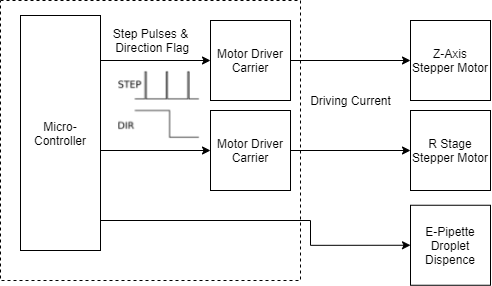
\includegraphics[width=0.4\textwidth]{img/ED_block_diag.png}
    \caption{Block Diagram of Base Electronic Design}
    \label{fig:e_block}
\end{figure}

\subsection{Motor}
\textit{Stepper motors allow for precise position control without the need for a feedback system and are capable of continuous rotation}
\subsection{Motor Drivers}

\begin{figure}[h]
    \centering
    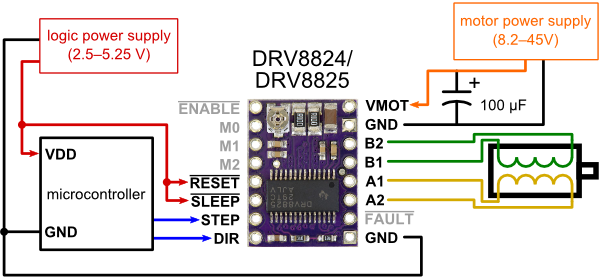
\includegraphics[width=0.45\textwidth]{img/stepper_driver schem_diagram.png}
    \caption{Minimal wiring diagram for DRV882x (full-step mode). \cite{pololu}}
\end{figure}

\subsection{Auxiliary Components}
\begin{itemize}
    \item Limit Switches
    \item Shaft Mounting Hubs 
\end{itemize}

\section{Initial Driving Firmware Implementation}
\subsection{Setup and Requirements}
With the parts selected and ordered, I wrote test firmware on an ESP32 to validate its ability in producing the required pulse train step signal to control the motor drivers. This produced signal, required to produce N steps (pulses) at a set average speed and ramp up and down that pulse speed and the head and tail of that signal.

Set values of 200 steps forward and back, at a speed of 200 steps per second, with max acceleration or 800 steps per second per second:

These pulses were captured on a second microcontroller listening for falling edges to trigger an interrupt routine to record and display that data.

\subsection{Results}

Figure \ref{fig:code}:a shows a successfully produced signal of 200 pulses with an inferred acceleration at its head/tail. This speed ramping is better illustrated in figure \ref{fig:code}:b showing the stepping change in pulses per second over the course of the pulse train.

\begin{figure}[h]
    \centering
    \begin{subfigure}{.45\textwidth}
      \centering
      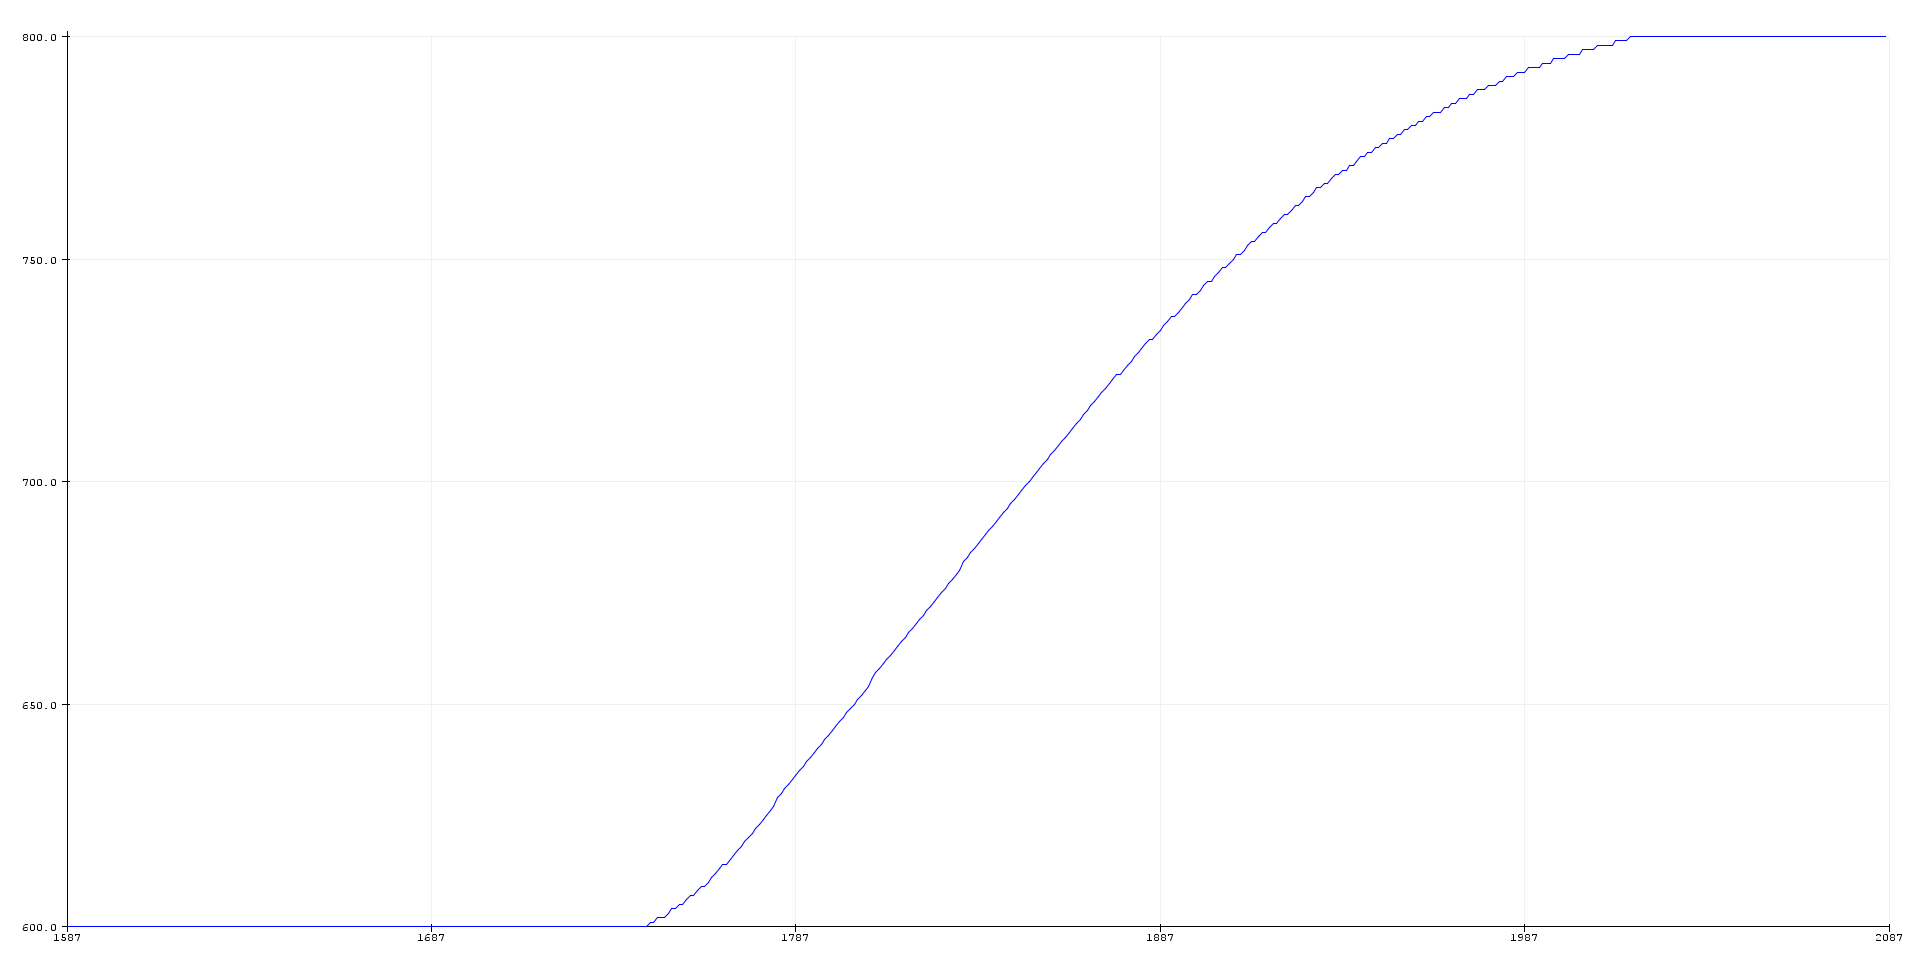
\includegraphics[width=\linewidth]{img/stepper_pulses.PNG}
      \caption{Pulse Count}
    \end{subfigure}%
    \begin{subfigure}{.45\textwidth}
      \centering
      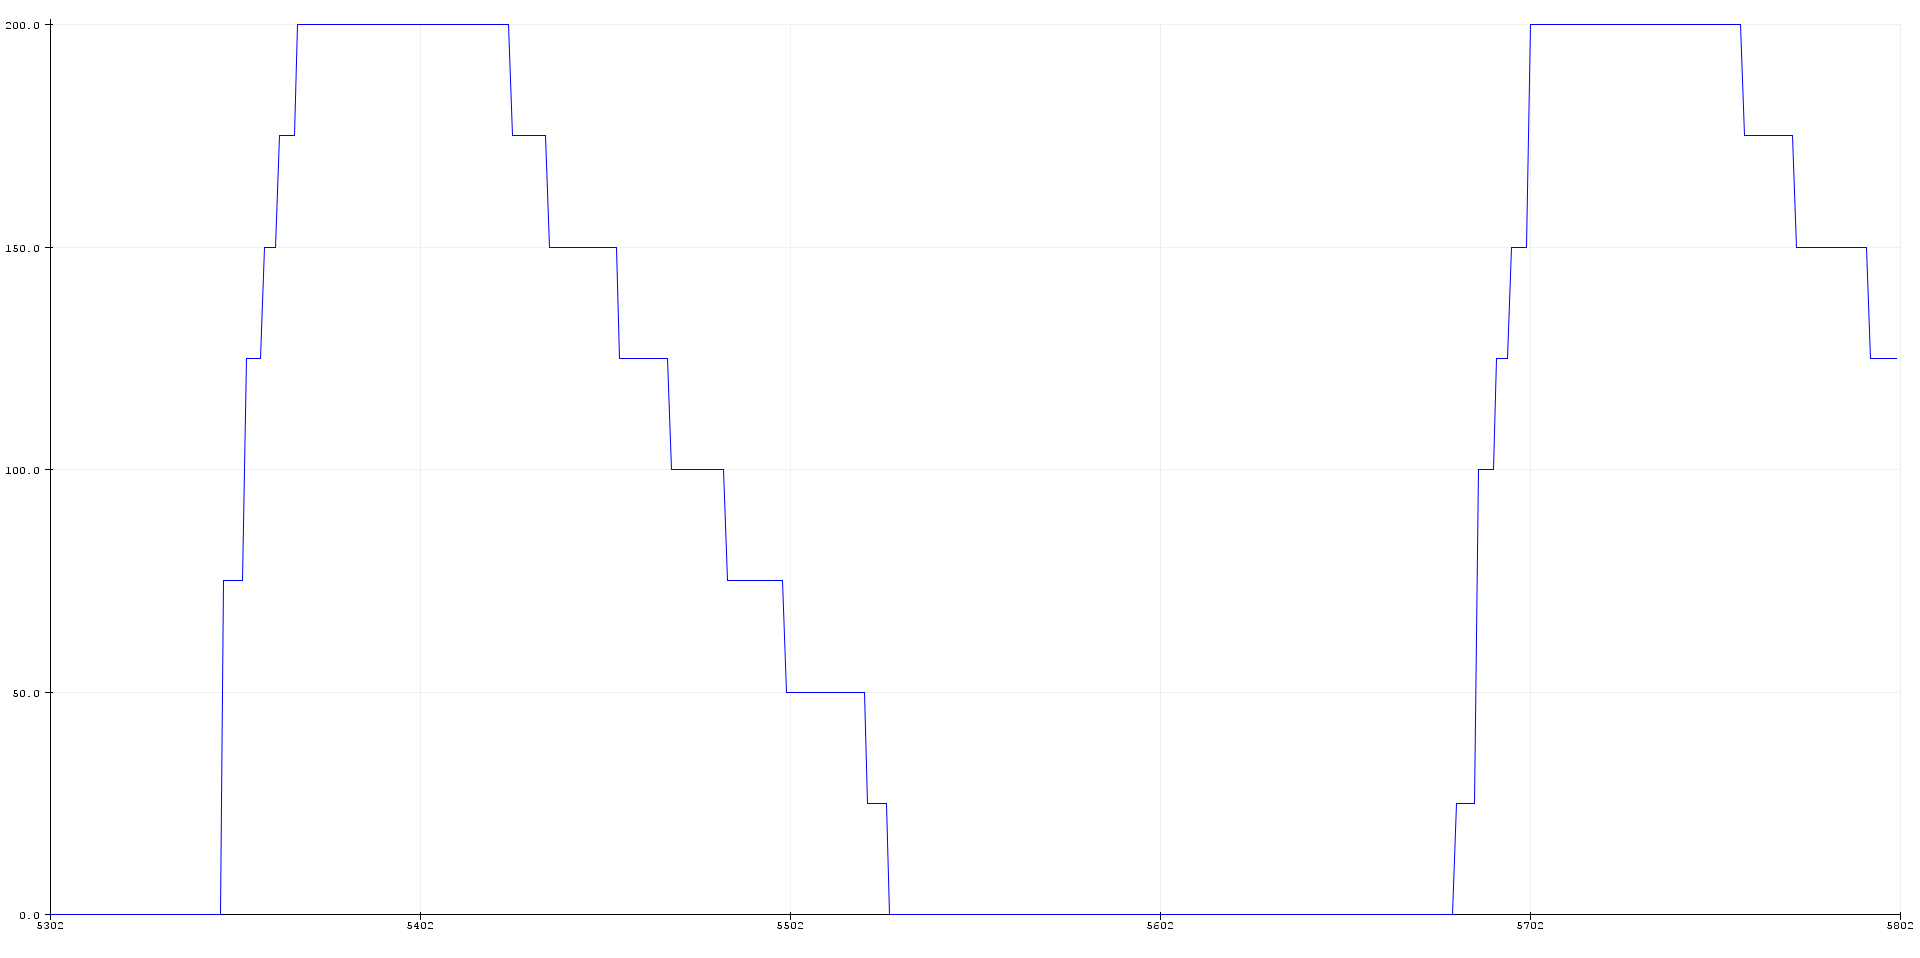
\includegraphics[width=\linewidth]{img/stepper_pulse_acc.PNG}
      \caption{Pulses per Second}
    \end{subfigure}
    \caption{}
    \label{fig:code}
  \end{figure}

  Upon the arrival of the motors themselves it will be determined what the exact requirements for this signal will be to prevent coil stalling and reduce vibrations in the system. It does however leave me with 3 main variables to tune this performance:
  \begin{itemize}
      \item Constant Step Count: What level of micro stepping can be achieved/whether it is required 
      \item Step speed: Limits, usable speeds, stability
      \item Step Acceleration: Motor performance, stall avoidance, resonances
  \end{itemize} 
